\documentclass{uni_tue_template}

\usepackage{color}
\usepackage[colorlinks]{hyperref}
\definecolor{darkred}{rgb}{0.5,0,0}
\definecolor{darkgreen}{rgb}{0,0.5,0}
\definecolor{darkblue}{rgb}{0,0,0.7}
\hypersetup{
			linkcolor={darkblue},
			filecolor={darkgreen},
			urlcolor={darkred},
			citecolor={darkblue},
}

\usepackage[export]{adjustbox}
\usepackage{tikz}
\usetikzlibrary{shapes}
\usepackage{rotating}
\usepackage{sistyle}

\lstdefinestyle{sql}{%
	language=SQL,%
	commentstyle=\color{comment},%
	stringstyle=\color{string},%
	keywordstyle=\color{keyword}\bfseries,%
	morekeywords={text, real, begin},%
	basicstyle=\ttfamily\footnotesize,%
	numbers=left,
	numberstyle=\tiny\color{black},
	stepnumber=1,
	showstringspaces=true,%
	columns=fixed,%
	moredelim=[is][\itshape]{@@}{@@},%
	tabsize=2
}
\lstset{aboveskip=-.6cm,style=sql, firstline=4}

\newcommand{\otext}[1]{\overset{\mathclap{\rule[-.3\baselineskip]{0pt}{0cm}\textmd{#1}}}}
\newcommand{\set}[1]{\mathbb{#1}}
\newcommand{\code}[1]{\texttt{{\footnotesize #1}}}
\newcommand{\md}[1]{\textmd{#1}}

% content of left head area e.g. subject like ETI
\def \headLeft{Andreas Schmied (3087156),\newline Tobias Stumpp (3798377)}

% content of center head area, used for names
\def \names{\"Ubungsblatt 8,\\ Datenbanksysteme II}

% content of right head area e.g. semester like WiSe 2012/13
\def \headRight{\today}

% set name for exercises
\def \exerciseName{Aufgabe}

\begin{document}
\exercise{}\\
\emph{Gegeben sei eine Relation, deren Tupel sich über 7 Seiten eines Heap-Files verteilen. Jede Page enthält dabei jeweils bis zu zwei einspaltige Tupel vom Typ (\code{INTEGER}). Die Seiten seien wie folgt befüllt:\\
\begin{center}
\vspace*{-1cm}
\begin{tabular}{|c|c|c|c|c|c|c|c|c|c|c|c|c|}
\cline{1-1}\cline{3-3}\cline{5-5}\cline{7-7}\cline{9-9}\cline{11-11}\cline{13-13}
(3),(4)& &(6),(2)& &(9),(4)& &(8),(7)& &(5),(6)& &(3),(1)& &(2),( )\\
\cline{1-1}\cline{3-3}\cline{5-5}\cline{7-7}\cline{9-9}\cline{11-11}\cline{13-13}
\end{tabular}
\end{center}
Sortieren Sie dieses File mit Hilfe des \emph{Two-Way Merge Sort Algorithmus}. Veranschaulichen Sie das Vorgehen des Algorithmus in dem Sie:}
\subExBegin{1{.}}
  \item \emph{Für alle Durchgänge die jeweils im Sekundärspeicher aufgebauten \emph{runs} angeben.\\}
  \begin{figure}[h!]
    \centering
    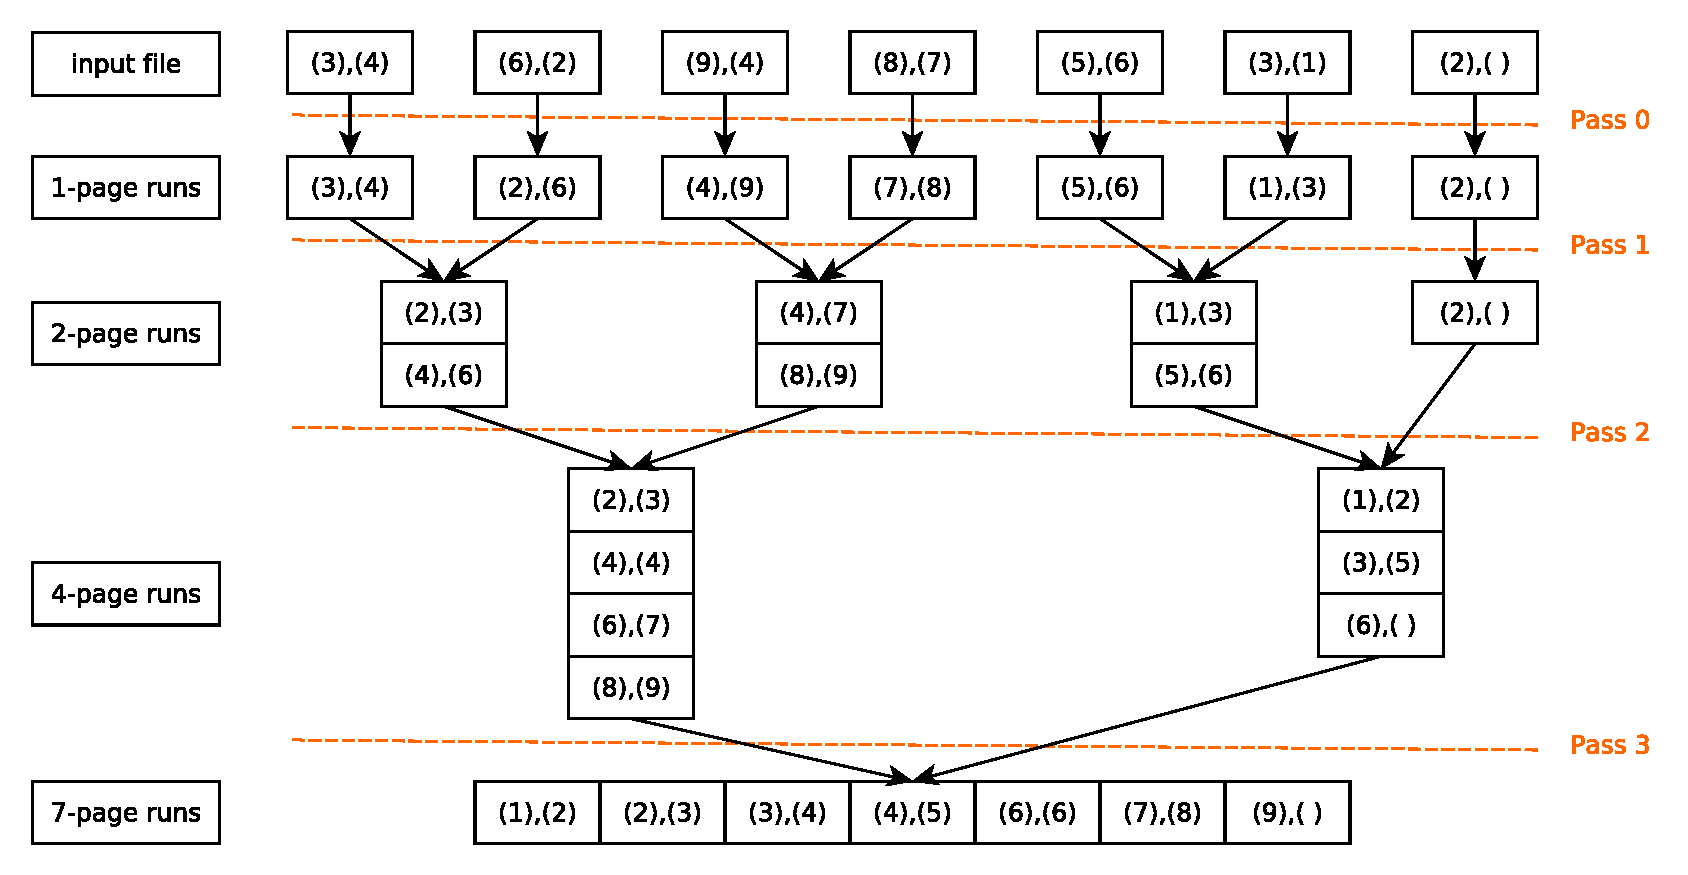
\includegraphics[scale=0.55]{graphml/01_1.pdf}
  \end{figure}
  \newpage
  \item \emph{Beispielhaft für die \emph{merges} von 2-page runs auf 4-page runs (\emph{Pass 2}), jeweils die Bufferbelegungen des benötigten, drei Seiten großen Hauptspeicherbereiches angeben.\\}
  Lösung unter der Annahme keiner paralleler Verarbeitung.
  \begin{center}
  \vspace*{-0cm}
  $\begin{array}{|c|c|c|cc|c|c|c|}
  \multicolumn{1}{c}{$Input1$}&\multicolumn{1}{c}{$Input2$}&\multicolumn{1}{c}{$Output$}&&\multicolumn{1}{c}{}&\multicolumn{1}{c}{$Input1$}&\multicolumn{1}{c}{$Input2$}&\multicolumn{1}{c}{$Output$}\\
  \multicolumn{1}{c}{\downarrow}&\multicolumn{1}{c}{\downarrow}&\multicolumn{1}{c}{\downarrow}&&\multicolumn{1}{c}{}&\multicolumn{1}{c}{\downarrow}&\multicolumn{1}{c}{\downarrow}&\multicolumn{1}{c}{\downarrow}\\
  \cline{1-3}\cline{6-8}
  (\ ),(\ )&(\ ),(\ )&(\ ),(\ )&&&(\ ),(\ )&(\ ),(\ )&(\ ),(\ )\\
    \cline{1-3}\cline{6-8}
  (2),(3)&(\ ),(\ )&(\ ),(\ )&&&(1),(3)&(\ ),(\ )&(\ ),(\ )\\
    \cline{1-3}\cline{6-8}
  (2),(3)&(4),(7)&(\ ),(\ )&&&(1),(3)&(2),(\ )&(\ ),(\ )\\
    \cline{1-3}\cline{6-8}
  (\ ),(3)&(4),(7)&(2),(\ )&&&(\ ),(3)&(2),(\ )&(1),(\ )\\
    \cline{1-3}\cline{6-8}
  (\ ),(\ )&(4),(7)&(2),(3)&&&(\ ),(3)&(\ ),(\ )&(1),(2)\\
    \cline{1-3}\cline{6-8}
  (\ ),(\ )&(4),(7)&(\ ),(\ )&&&(\ ),(3)&(\ ),(\ )&(\ ),(\ )\\
    \cline{1-3}\cline{6-8}
  (4),(6)&(4),(7)&(\ ),(\ )&&&(\ ),(\ )&(\ ),(\ )&(3),(\ )\\
    \cline{1-3}\cline{6-8}
  (\ ),(6)&(4),(7)&(4),(\ )&&&(5),(6)&(\ ),(\ )&(3),(\ )\\
    \cline{1-3}\cline{6-8}
  (\ ),(6)&(\ ),(7)&(4),(4)&&&(\ ),(6)&(\ ),(\ )&(3),(5)\\
    \cline{1-3}\cline{6-8}
  (\ ),(6)&(\ ),(7)&(\ ),(\ )&&&(\ ),(6)&(\ ),(\ )&(\ ),(\ )\\
    \cline{1-3}\cline{6-8}
  (\ ),(\ )&(\ ),(7)&(6),(\ )&&&(\ ),(\ )&(\ ),(\ )&(6),(\ )\\
    \cline{1-3}\cline{6-8}
  (\ ),(\ )&(\ ),(\ )&(6),(7)&&&(\ ),(\ )&(\ ),(\ )&(\ ),(\ )\\
    \cline{1-3}\cline{6-8}
  \end{array}$
  \end{center}
\subExEnd{}
%
\newpage 
%
\exercise{}\\
\emph{In der Vorlesung haben wir \emph{replacement sort} als Möglichkeit kenenn gelernt, um die Anzahl der initialen \emph{runs} des External Merge Sort Algorithmus noch weiter zu reduzieren. In dieser Aufgabe sollen Sie replacement sort in Java implementieren und testen.
\subExBegin{1{.}}
  \item Schreiben Sie ein Java-Programm, das replacement sort (nur \emph{Pass 0} des Sortieralgorithmus) implementiert. Als Parameter sollen Ihrem Programm die Größe des \emph{current set} (in Tupeln) und der Name der zu sortierenden Datei übergeben werden. Basierend auf diesen beiden Parametern, soll Ihr Proramm dann Dateien mit sortierten initialen \emph{runs} erzeugen. (Jede Zeile einer Datei entspricht dabei einer Page mit je einem Eintrag)
  \item Nutzen Sie Ihre Implementation um exemplarisch zu zeigen, dass replacement sort initial \emph{runs} erzeugt, die im Durchschnitt doppelt so groß wie dasd \emph{current set} sind (unter Annahme einer Gleichverteilung der zu sortierenden Eingabewerte).
\subExEnd{}}
\subExBegin{1{.}}
  \item Siehe Abgabe \code{assignment08.zip}
  \item Da ging wohl was schief :-/
\subExEnd{}

\end{document}